\subsection{تولید شرح بر تصاویر با استفاده از روش‌های مبتنی بر توجه بصری}
ایده‌ اصلی روش‌های مبتنی بر توجه بصری از پژوهش‌های موجود در زمینه ترجمه ماشینی گرفته شده است. این دسته از پژوهش‌ها مدلی ارائه می‌دهند که با استفاده از آن بتوان هر کلمه از جملات تولیدی را با تمرکز بر یک یا بخشی از کلمات موجود در جمله مبدا‌، تولید کرد. به طور مشابه، در حوزه تولید خودکار شرح بر تصاویر، از این دسته از پژوهش‌ها به منظور حصول مدلی استفاده می‌شود که قادر باشد هر یک از کلمات موجود در جمله را با استفاده از بخشی از تصویر ورودی، تولید نماید.
\\
در این فصل، ابتدا ایده اصلی ترجمه مبتنی بر توجه بصری را در حوزه ترجمه ماشینی ارائه خواهیم کرد و سپس کاربردهای این ایده را در حوزه تولید خودکار شرح بر تصاویر مورد بررسی قرار می‌دهیم. 

\subsection{روش‌های مبتنی بر توجه بصری در حوزه ترجمه ماشینی}

همان‌طور که گفته شد، تمام روش‌های قبلی را می‌توان به دو مرحله زیر تقسیم کرد.
\begin{enumerate}
\item نگاشت نمونه‌ها از فضای تصاویر به فضای ویژگي‌ها
\item نگاشت نمونه‌ها از فضای ویژگی‌ها به فضای جملات
\end{enumerate}

در حوزه ترجمه ماشینی، به تابع نگاشت مرحله اول، انکودر\enfootnote{Encoder} و به تابع نگاشت مرحله دوم، دیکودر\enfootnote{Decoder} گفته می‌شود. در این بخش، ما از این عبارات برای ارجاع به مراحل اول و دوم الگوریتم استفاده می‌نماییم.
\\
چارچوب کاری انکودر-دیکودر، در تعداد زیادی از پژوهش‌های حوزه ترجمه ماشینی به عنوان چارچوب کاری اصلی مورد استفاده قرار گرفته است. تمام روش‌های قبلی که در فصول قبل ذکر شد نیز از همین چارچوب کاری به عنوان چارچوب اصلی بهره برده‌اند. به عنوان مثال در روش‌های مبتنی بر یادگیری عمیق برای تولید خودکار شرح بر تصاویر از شبکه‌های عصبی کانولوشنی به طور معمول به عنوان انکودر و از شبکه‌های عصبی بازگشتی به عنوان دیکودر استفاده می‌شود.
\\
شکل \ref{fig:5-1} نشان‌دهنده ساختار کلی چارچوب کاری انکودر-دیکودر است.

\begin{figure}[h]
\centering
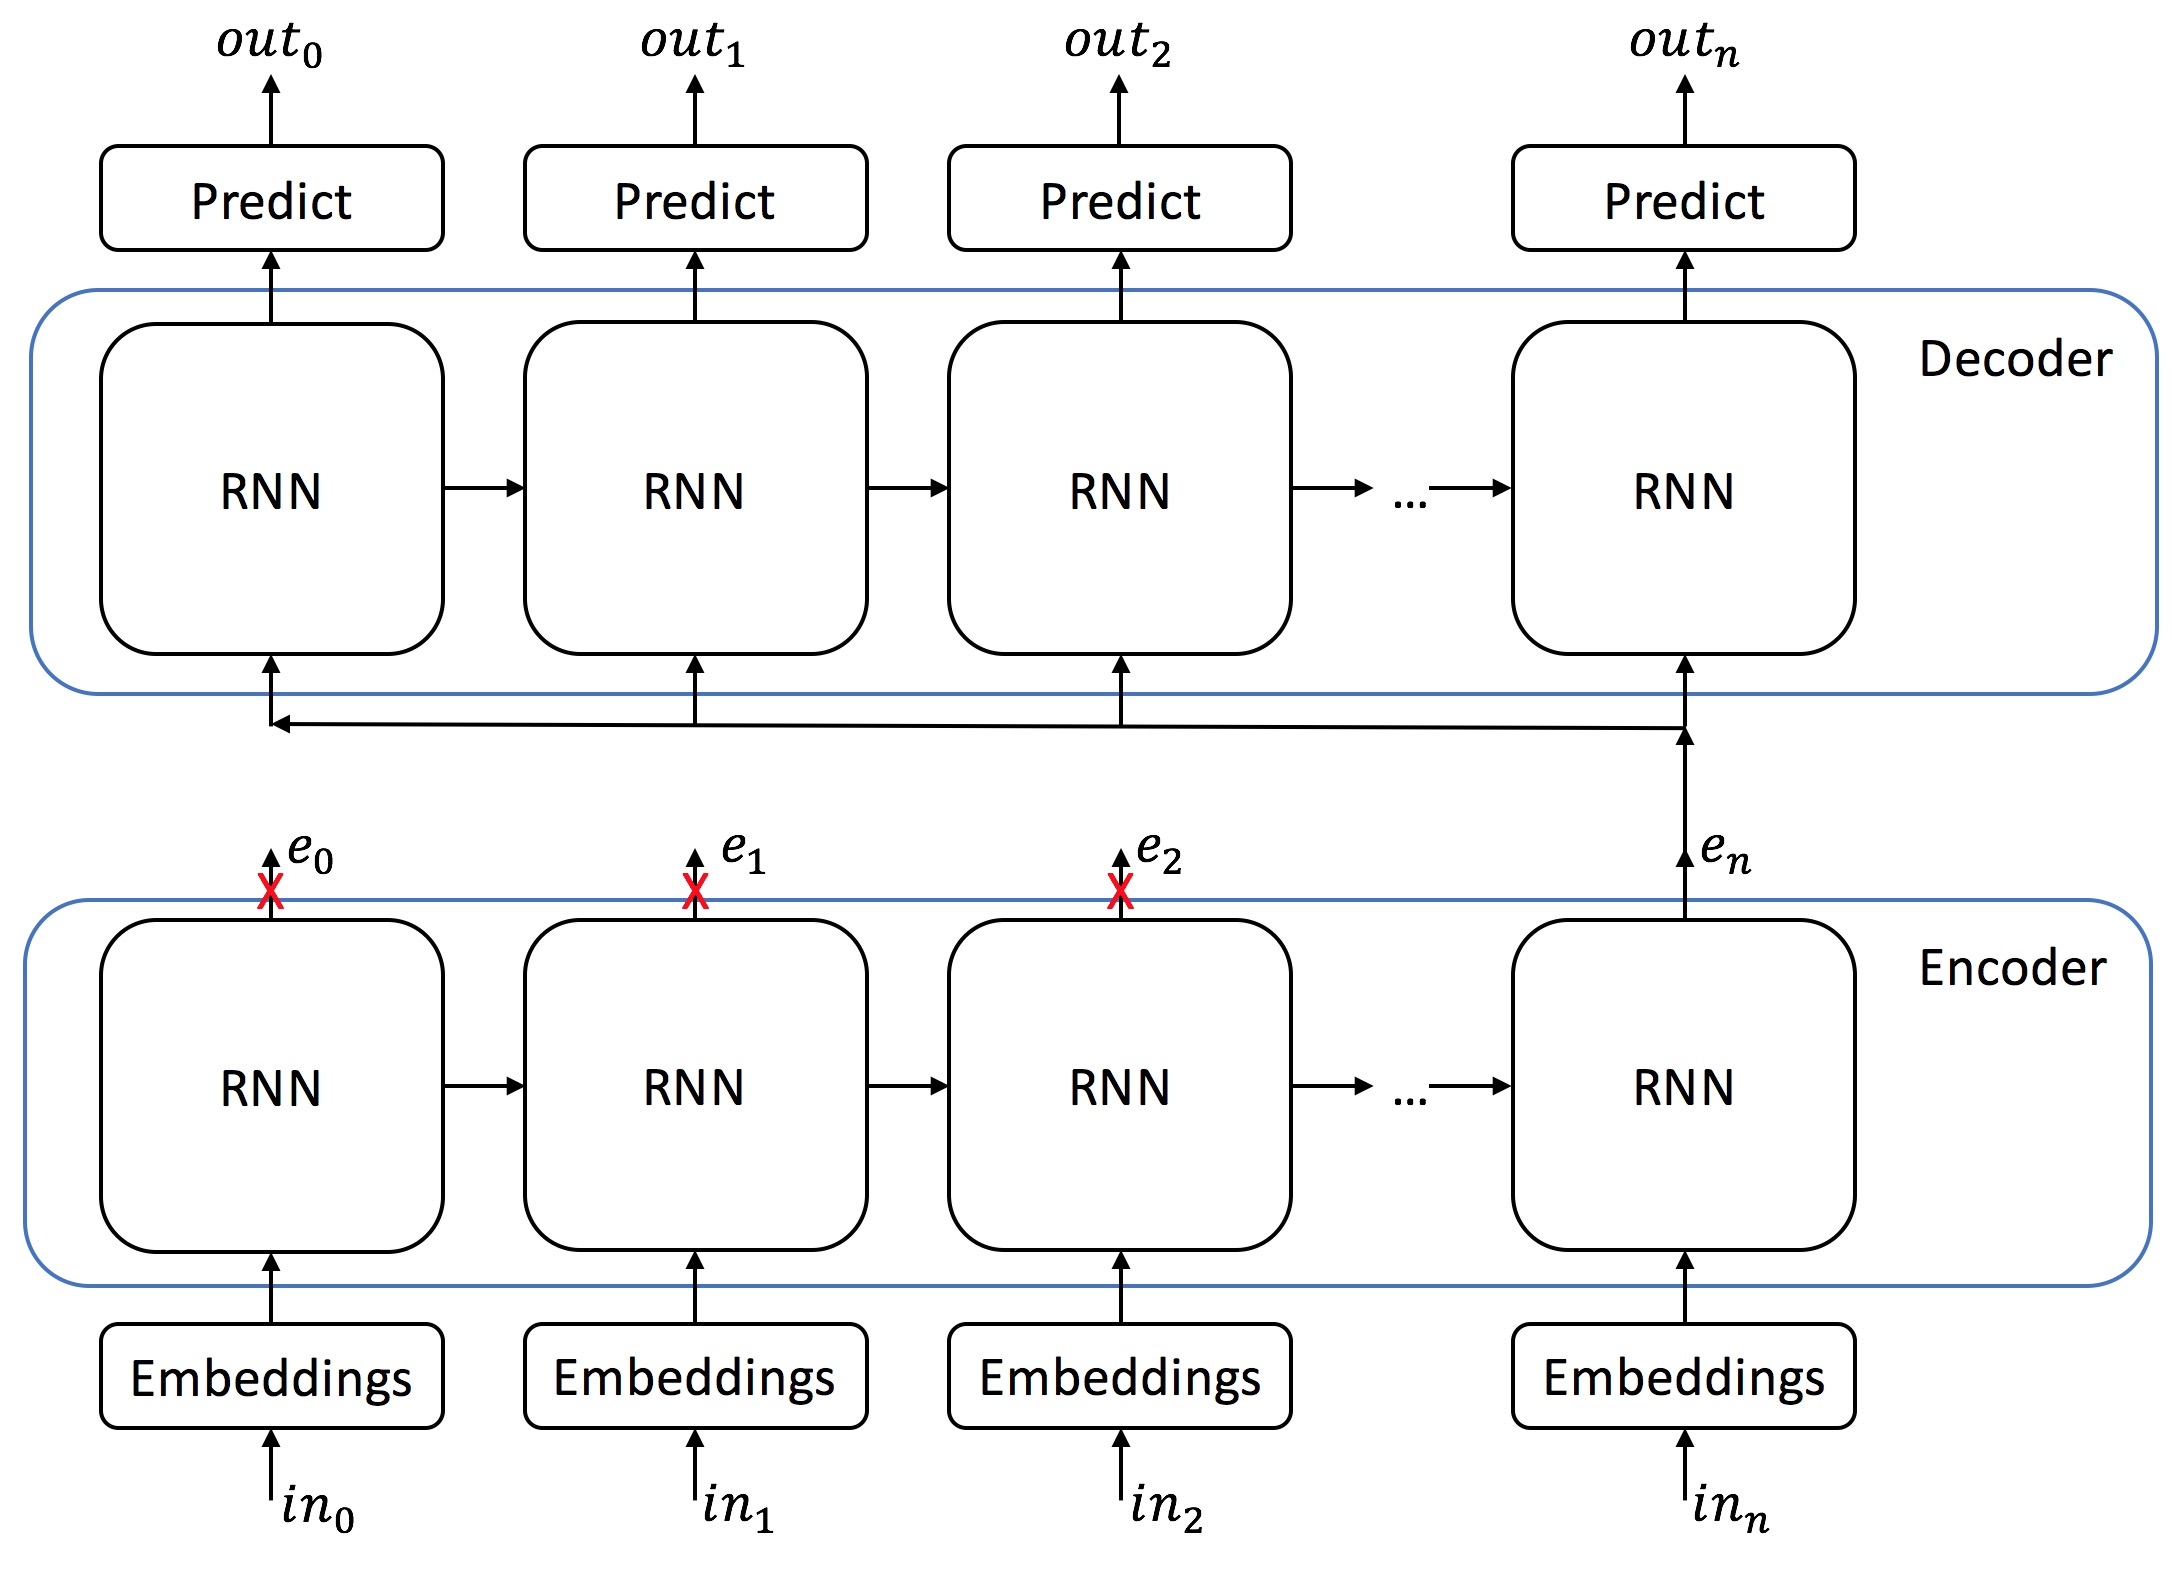
\includegraphics[scale=0.4]{Imgs/encoder-decoder.jpg}
\caption{ساختار کلی چارچوب کاری انکودر-دیکودر}
\label{ref:fig:5-1}
\end{figure}


در ادامه به بررسی بخش‌های مختلف این چارچوب کاری می‌پردازیم و سپس ایده اصلی روش‌های مبتنی بر توجه بصری را که توسط آقای بنجیو در پژوهش \cite{bahdanau2014neural} در سال 2014 ارائه شده است، مورد بررسی قرار خواهیم 
داد.


\subsubsection{انکودر}
 انکودر در این چارچوب کاری، با گرفتن یک جمله به عنوان ورودی، بردار ویژگی متناظر جمله مبدا را تولید می‌کند. جمله ورودی با دنباله‌ای از کلمات مدل می‌شود. همین‌طور هر کلمه را با یک بردار $n$ بعدی، که $n$ تعداد کلمات موجود در دیکشنری است، مدل می‌شود. به این ترتیب، هر جمله ورودی، یک بردار با طول متغیر است که هر مولفه آن خودش برداری به ابعاد  $n$ است. از طرفی بردار خروجی، که همان بردار ویژگی‌ها است، یک بردار با طول ثابت و قراردادی خواهد بود.
 \\
 عموما در کاربردهای ترجمه ماشینی در هر دو بخش انکودر و دیکودر از شبکه‌های عصبی بازگشتی استفاده می‌شود. در شبکه‌های عصبی بازگشتی، خروجی هر مرحله تابعی از ورودی آن مرحله و حالت شبکه در مرحله جاری است. با فرض این‌که $h_t$ حالت شبکه در زمان $t$ را نمایش دهد می‌توان رابطه تولید خروجی توسط شبکه عصبی بازگشتی را مطابق با \eqref{eq:5-1} تعریف نمود.
\begin{align*}
h_t& = f(X_t , h_{t-1}) \\
C& = q(h_1, \cdots, h_L)
\numberthis 
\label{eq:5-1}
\end{align*}
به طور معمول از شبکه 
\lr{LSTM}
 به عنوان تابع $f$ استفاده می‌شود و همین‌طور به جای استفاده از تابع $q$ حالت نهایی شبکه به عنوان بردار ویژگی مورد استفاده قرار می‌گیرد
\cite{bahdanau2014neural}.

\subsubsection{دیکودر}

 دیکودر به منظور نگاشت فضای ویژگی‌ها به فضای جملات مورد استفاده قرار می‌گیرد. خروجی انکودر، ورودی دیکودر است. با این فرض، ورودی دیکودر یک بردار ویژگی با طول ثابت است و خروجی آن که یک جمله به زبان مقصد است، همانند جمله مبدا، یک بردار با طول متغیر شامل بردارهای بازنمایی کلمات است. دیکودر در اصل در هر مرحله، به دنبال یافتن کلمه‌ای است که با داشتن کلمات تولید شده قبلی و بردار ویژگی موجود، محتمل‌ترین کلمه نسبت به بقیه کلمات موجود در دیکشنری باشد. تابع احتمال مربوطه را می‌توان به فرم \eqref{eq:5-2} تعریف نمود.
 
 \begin{equation}
 p(y_t | C, y_1, y_2, \cdots, y_{t-1}) = g(y_t, s_t, C)
 \label{eq:5-2}
 \end{equation}

در رابطه \eqref{eq:5-2}، $C$ نشان‌دهنده بردار ویژگی‌، $y_i$ نشان‌دهنده لغت $i$ام تولید شده از زبان مقصد و بردار $s_t$ نشان‌دهنده حالت شبکه بازگشتی مورد استفاده به عنوان دیکودر است.


 شکل \ref{fig:decoder} ساختار کلی دیکودر را نمایش می‌دهد.

\begin{figure}[h]
\centering
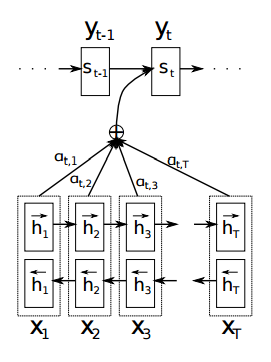
\includegraphics[scale=0.7]{Imgs/5-decoder.png}
\caption{ساختار دیکودر مورد استفاده در چارچوب کاری \cite{bahdanau2014neural}}
\label{fig:decoder}
\end{figure}

\subsubsection{ایده اصلی استفاده از توجه بصری}

همان‌طور که بیان شد، در چارچوب کاری انکودر-دیکودر، ابتدا جمله ورودی که شامل تعداد نامعلوم کلمه است به یک بردار با طول متغیر مدل می‌شود. بردار تولید شده توسط یک انکودر به یک بردار با طول ثابت، که همان بردار ویژگی‌ها است، نگاشت شده و در نهایت بردار ویژگی تولید شده توسط یک انکودر به یک بردار با طول متغیر که نماینده جمله زبان مقصد است، نگاشت می‌شود.
\\
فرآیند مذکور یک محدودیت جدی دارد و آن این است که انکودر باید بتواند تمام اطلاعات مورد نیاز برای تولید جمله را در یک بردار با طول ثابت بگنجاند و دیکودر باید بتواند تمام اطلاعات مورد نیاز خود را از همین بردار با موجود با طول ثابت، استخراج کند. این محدودیت باعث می‌شود قدرت کد کردن اطلاعات در بردار ویژگی کاهش یابد. برای حل این مشکل از ایده نقاط توجه استفاده می‌نماییم.
\\
در این دسته از روش‌ها به جای این‌که انکودر فقط یک بردار ویژگی تولید کند، بردارهای ویژگی مختلفی ایجاد می‌کند که هر بردار با تمرکز بر روی یک یا بخشی از جمله مبدا تولید شده است. به این ترتیب، هر بردار تولید شده شامل اطلاعات معنایی یک یا بخشی از جمله مبدا می‌باشد. به این طریق، دیکودر می‌تواند با انتخاب بین بردارهای معنایی تولید شده در هر مرحله، کلمه تولیدی را با تمرکز بر روی معنای یک کلمه و کلمات مجاور آن در جمله مبدا، تولید کند.
\\
در ادامه به بررسی تغییراتی که باید در انکودر و دیکودر اتفاق بیفتد تا بتوان به جای یک بردار ویژگی مجموعه‌ای از بردارهای ویژگی با تمرکز محلی ایجاد نمود و از آن‌ها برای تولید جمله استفاده نمود را مورد بررسی قرار می‌دهیم. برای سهولت فهم تغییرات، ابتدا تغییرات دیکودر را مطرح نموده و سپس به بررسی تغییرات انکودر خواهیم پرداخت.
\subsubsection{دیکودر در روش مبتنی بر توجه بصری}
فرض می‌کنیم به جای تنها یک بردار ویژگی، $L$ بردار ویژگی از ورودی استخراج شده باشد. آن‌ها را در یک ماتریس به شکل $C = [c_1, \cdots, c_L]^T$ بازنمایی می‌نماییم. فرض می‌کنیم بردار ویژگی $c_i$ به دنباله حاشیه‌نویسی‌های\enfootnote{Annotation} $h = [h_1, \cdots, h_L]^T$ وابسته است. حاشیه‌نویسی $h_i$ خود یک متغیر تصادفی به شکل برداری است که دارای دو ویژگی بسیار مهم می‌باشد.
\begin{enumerate}
\item .حاوی اطلاعات استخراج شده از تمام جمله است
\item تمرکز استخراج اطلاعات بر روی کلمه $i$ام و کلمات اطراف آن بوده است.
\end{enumerate}
با تعریف این دو ویژگی، حاشیه‌نویسی‌ها را می‌توان همان بردار ویژگی جمله تصور کرد با این شرط که علاوه بر این که معنای کل جمله را کد کرده‌اند، تمرکز بیشتری بر معنای کلمه $i$ام و کلمات مجاور آن دارند. به عبارت بهتر هر حاشیه‌نویسی علاوه بر این‌که معنای کلی جمله را کد می‌کند، حاوی معنای محلی مربوط به کلمات هم هست.
\\
با تعریف حاشیه‌نویسی به شکل فوق و با تکیه بر فرض‌های انجام شده، می‌توانیم مدل احتمالاتی ارائه شده را به شکل  \eqref{eq:5-3} تغییر دهیم. 
\begin{equation}
p(y_i| y_1, \cdots, y_{i-1}, X) = g(y_{i-1}, S_i, c_i)
\label{eq:5-3} 
\end{equation}
که در آن:
\begin{align*}
c_i = \Sigma_{j=1}^L \alpha_{ij}h_j
\numberthis
\label{eq:5-4}
\\
\alpha_{ij} = \frac{exp(e_{ij})}{\Sigma_{k=1}^Lexp(e_{ik})}
\numberthis
\label{eq:5-5}
\\
e_{ij} = f(s_{i-1}, h_j)
\numberthis
\label{eq:5-6}
\end{align*}

متغیر تصادفی $e_{ij}$ که در رابطه \eqref{eq:5-6} تعریف شده است نمایان‌گر میزان شباهت کلمه $i$ام در جمله خروجی به کلمه $j$ام در جمله ورودی است. وظیفه‌ این متغیر، هم‌ترازسازی\enfootnote{Alignment} ورودی و خروجی است. $\alpha_{ij}$ یک نرمال‌سازی روی امتیازهای محاسبه شده انجام می‌دهد. از این متغیر نرمال شده به عنوان وزن حاشیه‌نویسی‌ها استفاده می‌شود. مطابق با رابطه \eqref{eq:5-4} بردار ویژگی مورد استفاده برای تولید کلمه در جمله مقصد، از طریق یک میانگین‌گیری بر اساس وزن معنایی کلمات تولید می‌شود.
\\
در رابطه \eqref{eq:5-6} $s_{i-1}$ بردار حالت شبکه دیکودر در زمان $i-1$ و $f$ یک تابع امتیاز است. تابع امتیاز مورد استفاده در این رابطه را می‌توان با یک شبکه عصبی پیش‌رو\enfootnote{Feed Forward Neural Network} مدل‌سازی کرد. در صورت استفاده از شبکه عصبی پیش‌رو برای مدل‌سازی تابع شباهت، در صورتی که از هم‌ترازسازی نرم\enfootnote{Soft Alignment} استفاده شود، تابع هدف مشتق‌پذیر شده و می‌توانیم از الگوریتم پس‌انتشار خطا برای آموزش استفاده نماییم.


\subsubsection{انکودر در روش مبتنی بر توجه بصری}
برای طراحی انکودر در این بخش، باید مکانیزمی ارائه شود که قادر باشد حاشیه‌نویسی‌های $h_1$ تا $h_L$ را طوری تولید کند که دو شرط مطرح شده در بخش قبلی را ارضا نمایند. به عبارت دیگر باید بردارهای ویژگی‌ای استخراج نماییم که علاوه بر این‌که حاوی معنای کل جمله باشند، هر یک از آن‌ها بر روی معنای یک کلمه و کلمات اطراف آن تمرکز بیشتری نسبت به سایر بردارها داشته باشند تا بتوانیم علاوه بر مدل‌سازی معنای کلی جمله، از معنای محلی کلمات هم استفاده نماییم.
\\
به این منظور از یک شبکه عصبی بازگشتی دوطرفه در مدل‌سازی انکودر استفاده می‌نماییم. شکل \ref{fig:biencoder} ساختار کلی یک شبکه عصبی بازگشتی دوطرفه را نمایش می‌دهد. 

\begin{figure}[h]
\centering
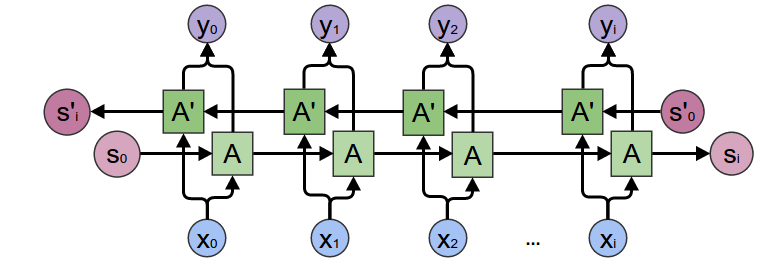
\includegraphics[scale=0.6]{Imgs/biencoder.png}
\caption{ساختار کلی یک شبکه عصبی بازگشتی دوطرفه}
\label{fig:biencoder}
\end{figure}

همان‌طور که در شکل \ref{fig:biencoder} مشخص است، یک شبکه عصبی بازگشتی دوطرفه شامل دو شبکه پیش‌رو در خلاف جهت یک‌دیگر است. حالت‌های مخفی شبکه پیش‌رو رو به راست را با $h_i^\rightarrow$ و حالت‌های مخفی شبکه پیش‌رو رو به چپ را با $h_i^\leftarrow$ نمایش می‌دهیم. همان‌طور که در شکل پیداست، خروجی‌های شبکه در این ساختار هم به حالت‌های سمت راست و کلمات سمت راست در جمله و هم به حالات و کلمات سمت چپ وابسته هستند. پس همین خروجی‌ها را می‌توان به عنوان حاشیه‌نویسی‌هایی که هر دو ویژگی را دارند مورد استفاده قرار داد.
	یکی از راه‌های ساده برای ایجاد حاشیه‌نویسی با استفاده از حالات شبکه‌های پیش‌رو رو به راست و رو به چپ این است که مطابق با رابطه \eqref{eq:5-7} با پشت سر هم قرار دادن حالات شبکه، حاشیه‌نویسی مورد نیاز را تولید نماییم.
	\begin{equation}
	h_j = [{h_j^\rightarrow}^T, {h_j^\leftarrow}^T]^T
	\label{eq:5-7}
	\end{equation}



\subsection{روش‌های مبتنی بر توجه بصری در حوزه تولید شرح متناظر تصویر}
در بخش قبل به بیان ایده اصلی روش‌های مبتنی بر توجه بصری در حوزه ترجمه ماشینی پرداختیم. ساختار کلی انکودرها و دیکودرها در این قالب و همین‌طور نحوه تولید بردارهای ویژگی مختلف از جمله مبدا و استفاده از این بردارها در تولید جمله مقصد را مورد بررسی قرار دادیم. در این بخش  به بررسی پژوهش‌هایی خواهیم پرداخت که از این ایده در حوزه تولید شرح متناظر تصویر بهره‌ جسته‌اند.
\\
یکی از برجسته‌ترین و مورد توجه‌ترین پژوهش‌ها از این دست، پژوهشی است که آقای بنجیو و همکارانش در سال 2015 ارائه داده‌اند
\cite{xu2015show}.
در این بخش به بررسی این پژوهش خواهیم پرداخت.

\subsubsection[تولید شرح متناظر تصویر با استفاده از توجه بصری و شبکه‌های عصبی]{تولید شرح متناظر تصویر با استفاده از توجه بصری و شبکه‌های عصبی \cite{xu2015show}}
	
در این پژوهش که در سال 2015 توسط آقای بنجیو و همکارانش ارائه شده است از ایده استفاده از توجه در حوزه ترجمه ماشینی استفاده شده است تا شرح متناظر تصاویر با دقت بیشتری تولید شود. چارچوب کاری انکودر-دیکودر مانند آن‌چه در بخش قبلی مطرح شد در این پژوهش مورد استفاده قرار گرفته است.
\\
انکودر ارائه شده در این پژوهش، یک شبکه عصبی کانولوشنی است که قادر به تولید $L$ بردار ویژگی مختلف است. به هر یک از این بردارهای ویژگی یک حاشیه‌نویسی\enfootnote{Annotation} تصویر گفته می‌شود. بردارهای حاشیه‌نویسی، همان‌طور که در بخش قبل ذکر شد، باید دارای دو شرط زیر باشند:
\begin{enumerate}
\item حاوی معنای تصویر به طور کلی باشند.
\item تمرکز بیشتری روی یکی از بخش‌های تصویر داشته باشند.
\end{enumerate}
برای این‌که بتوانیم دو شرط فوق را در بردارهای حاشیه‌نویسی تولید شده از انکودر بگنجانیم از خروجی لایه ما قبل آخر شبکه عصبی کانولوشنی به عنوان بردارهای حاشیه‌نویسی استفاده می‌کنیم. هر بردار حاشیه‌نویسی یک بردار $D$ بعدی است که مربوط به یک بخش از تصویر می‌شود و آن را با $a_i$ نمایش می‌دهیم. بنابر این داریم:
\begin{equation}
a = \{a_1, a_2, \cdots, a_L\}, a_i \in R^D
\end{equation}

در این پژوهش از یک شبکه حافظه کوتاه‌مدت بلند به عنوان دیکودر استفاده شده است. این شبکه با دریافت مجموعه بردارهای حاشیه‌نویسی $a$، جمله‌ای به زبان انگلیسی تولید می‌کند که شامل دنباله‌ای از $C$ کلمه است. هر کلمه با یک بردار $K$ بعدی نمایش داده می‌شود که $K$ تعداد کلمات موجود در دیکشنری است. در هر یک از بردارهای بازنمایی کلمات فقط یک مولفه یک است و مابقی مولفه‌ها صفر هستند. مولفه‌ای که برابر با یک است نمایش‌دهنده اندیس کلمه در دیکشنری است.
\\
شکل \ref{fig:satenc} یک سلول از شبکه حافظه کوتاه‌مدت بلند مورد استفاده در این پژوهش به عنوان دیکودر را نمایش می‌دهد. 
\begin{figure}[h]
\centering
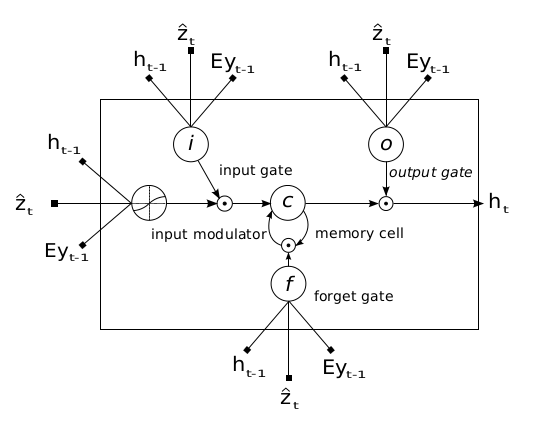
\includegraphics[scale=0.6]{Imgs/satenc.png}
\caption{یک واحد از شبکه حافظه کوتاه‌مدت بلند مورد استفاده در دیکودر پژوهش \cite{xu2015show}}
\label{fig:satenc}
\end{figure}
روابط مربوط به یادگیری این شبکه را می‌توان مطابق با روابط \eqref{eq:5-8} تا \ref{eq:5-13}  نمایش داد. در همه روابط، تابع $T$ یک تابع نگاشت خطی به شکل $T: R^{D+m+n}*R^n$ است که پارامترهای آن آموزش داده‌ شده‌اند. متغیر $i_t$ ورودی، $f_t$ خروجی سلول فراموشی، $c_t$ حافظه، $o_t$ خروجی و $h_t$ حالت مخفی شبکه را نمایش می‌دهند. 
\begin{align*}
i_t &= \sigma(T(Ey_{t-1}, h_{t-1}, \hat{z}_{t-1})) \numberthis \label{eq:5-8} \\
f_t &= \sigma(T(Ey_{t-1}, h_{t-1}, \hat{z}_{t-1})) \numberthis \label{eq:5-9} \\
o_t &= \sigma(T(Ey_{t-1}, h_{t-1}, \hat{z}_{t-1})) \numberthis \label{eq:5-10} \\
g_t &= \sigma(T(Ey_{t-1}, h_{t-1}, \hat{z}_{t-1})) \numberthis \label{eq:5-11} \\
c_t &= f_t \odot c_{t-1} + i_t \odot g_t \numberthis \label{eq:5-12} \\
h_t &= o_t \odot tanh(c_t) \numberthis \label{eq:5-13} \\
\end{align*}

بردار $\hat{z}_{t-1}$ بردار معنای تصویر را نمایش می‌دهد که با استفاده از بردارهای حاشیه‌نویسی تولید شده در انکودر تولید می‌شود. ماتریس $E$، ماتریس جانمایی\enfootnote{Embedding Matrix} به ابعاد $m * K$ است. تابع $\sigma$ تابع فعالیت سیگموئیدی و $\odot$ حاصل‌ضرب مولفه‌های نظیر به نظیر بردارها را نمایش می‌دهند.
\\
فرایند آموزش دیکودر کاملا مطابق با فرایند آموزش معمول شبکه حافظه کوتاه‌مدت بلند است. تنها تفاوت در این پژوهش وجود و نحوه محاسبه بردار معنای $\hat{z}_{t-1}$  است که توجه بصری را تعریف می‌کند. برای محاسبه این متغیر تابع $\phi$ را تعریف می‌نماییم. این تابع در هر لحظه از زمان با استفاده از مجموعه بردارهای حاشیه‌نویسی $a$ برداری تولید می‌کند که به عنوان بردار ویژگی‌ استخراج شده از تصویر در هر لحظه مورد استفاده قرار می‌گیرد.
\\
تابع $phi$ می‌تواند به دو شکل بردار ویژگی را تولید نماید. روش اول این است که ابتدا با تولید وزن‌های مثبت $\alpha_i$ برای هر ناحیه از تصویر با بردار حاشیه‌نویسی $a_i$ یک احتمال برای میزان مناسب بودن ناحیه $i$ از تصویر برای استفاده در تولید کلمه در زمان $t$ تعریف شود. سپس بردار حاشیه‌نویسی با بیشترین احتمال برای تولید کلمه انتخاب شده و به مراحل بعدی ارسال شود. این روش را تحت عنوان روش توجه سخت\enfootnote{Hard Attention} نام‌گذاری می‌نماییم.
\\
روش دوم برای تولید بردار ویژگی تصویر در هر لحظه توسط تابع $\phi$ این است که اعداد مثبت تولید شده $\alpha_i$ را به طور مستقیم به عنوان معیاری جهت سنجش میزان مناسب‌بودن نسبی نواحی نسبت به یک‌دیگر مورد استفاده قرار دهیم و با استفاده از یک میانگین‌گیری وزن‌دار بر حسب همین وزن‌های مثبت از بردارهای حاشیه‌نویسی اقدام به تولید بردار ویژگی تصویر نماییم. به این روش، روش توجه نرم \enfootnote{Soft Attention} می‌گوییم.
\\
به جهت سهولت در امر رابطه‌بندی توجه بصری در فرایند آموزش انکودر و دیکودر، متغیر تصادفی $s_{t.i}$ را معرفی می‌نماییم که نشان‌دهنده این است که آیا در زمان $t$، از بردار ویژگی مربوط به ناحیه $i$ام تصویر، برای تولید کلمه استفاده می‌شود یا خیر. اگر در زمان $t$ از بردار ویژگی ناحیه $i$ام، که همان بردار حاشیه‌نویسی با اندیس $i$ است، به منظور تولید کلمه استفاده شود، مقدار متغیر $s_{t,i}$ برابر با یک و در غیر این‌ صورت برابر با صفر قرار می‌‌گیرد.
\\
با استفاده از متغیر تصادفی تعریف شده می‌توان به راحتی روابط مربوط به مدل‌سازی توجه بصری نرم و سخت را به شرح زیر تشکیل داد. نکته آخر این‌که در پژوهش مورد بررسی، به منظور تولید احتمال کلمه بعدی با توجه به کلمات تولید شده قبلی و بردار ویژگی استخراج شده از تصویر از رابطه \eqref{eq:5-131} استفاده شده است.
\begin{equation}
p(Y_t | a, Y_1^{t-1}) \propto exp(L_o(EY_{t-1} + L_h h_{t} + L_z \hat{z}_t)) 
\label{eq:5-131}
\end{equation}
در رابطه \eqref{eq:5-13} ماتریس‌های $L_o \in R^{K*m}$، $L_h \in R^{m*n}$، $L_z \in R^{m*d}$ و $E$ پارامترهای شبکه هستند که باید آموزش داده شوند.

\begin{enumerate}
\item \textbf{توجه بصری سخت} \\
با فرض یک توزیع \lr{Multinoulli} مطابق رابطه \eqref{eq:5-hatmult} می‌توان متغیر $\hat{z}_t$ را به عنوان بردار ویژگی استخراج‌شده نهایی با توجه به بردارهای حاشیه‌نویسی $a$ و توجه بصری بصری، به شکل رابطه \eqref{eq:5-hat} محاسبه نمود.

\begin{align*}
&p(s_{t,i} = 1 | s_{j<t}, a) = \alpha_{t,i}
\numberthis \label{eq:5-hatmult} \\
&\hat{z}_t = \Sigma_t s_{t,i} a_i
\numberthis \label{eq:5-hat} 
\end{align*}

برای آموزش وزن‌های شبکه یک تابع هدف به نام $L_s$ مطابق با رابطه \eqref{eq:5-hl} مطرح می‌شود که یک کران پایین از بیشینه درستنمایی $p(Y | a)$ است که در آن $Y$ دنباله کلمات تولید شده نهایی و 
$a$ بردارهای حاشیه‌نویسی تولید شده از روی تصویر را نمایش می‌دهند.

\begin{align*}
log\>p(Y | a) = log\> \Sigma_s\> p(s | a) p(Y | s, a) \>\geq\> \Sigma_s\> p(s | a) \>log\> p(Y | s, a) = L_s \numberthis \label{eq:5-hl} \\ 
\end{align*}

با ارائه تابع هدف $L_s$ مطابق با رابطه \eqref{eq:5-hl} و بهینه‌سازی آن می‌توان رابطه به‌روزرسانی وزن‌ها در فرایند آموزش را محاسبه نمود. رابطه \eqref{eq:5-hardatten1} محاسبات مربوطه را نمایش می‌دهد.

\begin{align*}
\frac{\partial L_s}{\partial W} = \Sigma_s p(s|a) [\frac{\partial \> log \> p(Y| s, a)}{\partial W} + log \> p(Y|s,a)\frac{\partial \> log \> p(s|a)}{\partial W}] \numberthis \label{eq:5-hardatten1}
\end{align*}

به جای متغیر $s_t$ در رابطه \eqref{eq:5-hardatten1} می‌توان با استفاده از روش نمونه‌برداری مونت‌کارلو\enfootnote{Monte Carlo Sampling} نمونه‌های تصادفی $\tilde{s_t}$ تولید کرد و سپس با استفاده از رابطه \eqref{eq:5-hardatten2} تابع هدف را بهینه نمود. 
\begin{equation}
\frac{\partial \> L_s}{\partial W} \approx \frac{1}{N} \Sigma_{n=1}^N [\frac{\partial \> log \> p(Y|\tilde{s}^n , a)}{\partial W} + log \> p (Y| \tilde{s}^n , a) \frac{\partial \> log \> p(\tilde{s}^n | a)}{\partial W}]
\label{eq:5-hardatten2}
\end{equation}
	
\item \textbf{توجه بصری نرم} \\

همان‌طور که گفته شد، تولید بردار ويژگی را می‌توان با میانگین‌گیری وزن‌دار روی بردارهای حاشیه‌نویسی انجام داد. در شرایطی که وزن‌های تخصیص داده شده به بردارهای حاشیه‌نویسی برابر صفر نباشند، توجه بصری نرم، فرایندی خواهد بود شامل تولید بردار ویژگی با استفاده از تمام حاشیه‌نویسی‌های موجود و با تمرکز روی تعدادی از حاشیه‌نویسی‌ها که ضریب بیشتری دارند. از آنجا که این شیوه محاسبه بردار ویژگی شامل یک بردار میانگین‌گیری وزن‌دار است، تمام تابع هدف مشتق‌پذیر شده و امکان استفاده از روش پس‌انتشار خطا برای یادگیری وزن‌ها فراهم می‌شود.
\\
در این روش به طور کلی می‌توان بردار ویژگی $\hat{z}_t$ را مطابق با رابطه \eqref{eq:5-soft1} محاسبه نمود.

\begin{equation}
E_{p(s_t | a)} [\hat{z}_t] = \Sigma_{i=1}^L \alpha_{t,i} a_i
\label{eq:5-soft1}
\end{equation}

مطابق با رابطه \eqref{eq:5-11} حالت مخفی شبکه یک ترکیب خطی از بردار ویژگی استخراج شده از تصویر به همراه یک غیرخطی‌سازی با استفاده از تابع $tanh$ است. برای تقریب مرتبه اول حالت مخفی شبکه می‌توان از امید ریاضی بردار ویژگی $\hat{z}_t$ در رابطه \eqref{eq:5-11} استفاده کرد. با در نظر گرفتن رابطه \eqref{eq:5-13} می‌توان متغیر $n_t$ را به شکل 
$n_t = L_o (EY_{t-1} + L_h h_t + L_z \hat{z}_t) $
تعریف نمود. با این تعریف،‌ متغیر $n_{t,i}$ مشخص‌کننده متغیر $n_t$ است در شرایطی که $\hat{z}_t = a_i$ باشد. با استفاده از متغیر تعریف شده، میانگین هندسی وزن‌دار نرمال‌شده \enfootnote{Normalized Weighted Geometric Mean (NWGM)} را برای تولید کلمه $k$ام مطابق با رابطه \eqref{eq:5-nwgm} تعریف می‌نماییم.

\begin{equation}
NWGM[P(y_t = k | a)] = \frac{\Pi_i exp(n_{t,k,i})^{p(s_{t,i} = 1 | a)}}{\Sigma_j \Pi_i exp(n_{t,j,i})^{p(s_{t,i} = 1 | a)}} = \frac{exp(E_{p(s_{t,i}|a)}[n_{t,k}])}{\Sigma_j exp(E_{p(s_{t,i}|a)}[n_{t,j}])}
\label{eq:5-nwgm}
\end{equation}

از آنجا که 
$E[n_t] = L_o(EY_{t-1} + L_h E[h_t] + L_z E[\hat{z}_t])$
، متغیر $NWGM$ می‌تواند به خوبی توسط بردار ویژگی $\hat{z}_t$ تخمین زده شود. این بدین معناست که میانگین هندسی وزن‌دار نرمال‌شده لایه نهایی شبکه می‌تواند با اعمال تابع $soft\>max$ به امید ریاضی ترکیبات خطی لایه‌های پایین‌تر محاسبه شود. 


\end{enumerate}


آزمایشات انجام شده در این پژوهش روی سه مجموعه‌داده
 \lr{Flickr8k}،
\lr{Flickr30k} و
 \lr{Microsoft COCO}
  اجرا شده است که به ترتیب شامل 8000، 30000 و 82783 تصویر با شرح تولید‌شده توسط عوامل انسانی هستند. دو مجموعه‌داده اول برای هر تصویر، 5 شرح مختلف و مجموعه‌داده سوم در برخی تصاویر بیش از ۵ شرح را شامل می‌شوند. در تمام پژوهش‌ها به منظور یکسان‌سازی آزمایشات و نتایج، از ۵ شرح برای هر تصویر استفاده شده است. 
  \\
  هر دو نوع محاسبه توجه بصری در این پژوهش مورد آزمایش قرار گرفته‌اند و نتایج هریک به طور جداگانه بیان شده است. در این پژوهش از معیارهای \lr{BLEU} و \lr{METEOR} به منظور ارزیابی مدل استفاده شده است.
  \\
همان‌طور که در جدول \ref{tbl:5-xures} مشخص است، در هر سه مجموعه‌داده،‌ پژوهش \cite{xu2015show} بهترین عملکرد را نسبت به روش‌های دیگر از خود نشان داده است. استفاده از توجه بصری نرم در مجموعه‌داده‌های \lr{Flickr30k} و \lr{MS COCO} عمل‌کرد بهتری نسبت به روش‌های دیگر از لحاظ معیار \lr{METEOR} از خود نشان داده‌ است. همین‌طور استفاده از توجه بصری سخت، بهترین عملکرد را در معیار \lr{BLEU} از خود نشان داده است.
\\
یکی از فعالیت‌های مفید برای بررسی نحوه عملکرد مدل که در این پژوهش مورد استفاده قرار گرفته است، بصری کردن فرایند تولید کلمه توسط مدل است. در این پژوهش، توجه بصری روی تصویر در هر مرحله به همراه کلمه تولید شده در هر مرحله مشخص شده‌اند که در درک نحوه عمل‌کرد مدل و همین‌طور پیدا کردن دلایل ایجاد کلمات غیر مرتبط بسیار کمک‌کننده هستند.  

  
\begin{table}[h]
\centering
\caption{نتایج اعمال روش \cite{xu2015show} بر روی مجموعه‌داده‌های مختلف در مقایسه با روش‌های مختلف. \cite{xu2015show}}
\label{tbl:5-xures}
\begin{tabular}{| c | c | c | c | c | c | c |}
\hline
مجموعه‌داده & نام مدل & \lr{BLEU-1} & \lr{BLEU-2} & \lr{BLEU-3} & \lr{BLEU-4} & \lr{METEOR} 
\\
\hline
\hline
\lr{Flickr8k} & \lr{Google NIC} & 63.0 & 41.0 & 27.0 & \lr{--} & \lr{--} 
\\
\lr{Flickr8k} & \lr{Log Bilinear} & 65.6 & 42.4 & 27.7 & 17.7 & 17.31 
\\
\lr{Flickr8k} & \lr{Soft Attention} & \textbf{67.0} & 44.8 & 29.9 & 19.5 & 18.93 
\\
\lr{Flickr8k} & \lr{Hard Attention} & \textbf{67.0} & \textbf{45.7} & \textbf{31.4} & \textbf{21.3} & \textbf{20.30} 
\\
\hline
\lr{Flickr30k} & \lr{Google NIC} & 66.3 & 42.3 & 27.7 & 18.3 & \lr{--} 
\\
\lr{Flickr30k} & \lr{Log Bilinear} & 60.0 & 38.0 & 25.4 & 17.1 & 16.88 
\\
\lr{Flickr30k} & \lr{Soft Attention} & 66.7 & 43.4 & 28.8 & 19.1 & \textbf{18.49} 
\\
\lr{Flickr30k} & \lr{Hard Attention} & \textbf{66.9} & \textbf{43.9} & \textbf{29.6} & \textbf{19.9} & 18.46 
\\
\hline
\lr{MS COCO} & \lr{CMU/MS Research} & \lr{--} & \lr{--} & \lr{--} & \lr{--} & 20.41 
\\
\lr{MS COCO} & \lr{MS Research} & \lr{--} & \lr{--} & \lr{--} & \lr{--} & 20.71
\\
\lr{MS COCO} & \lr{BRNN} & 64.2 & 45.1 & 30.4 & 20.3 & \lr{--} 
\\
\lr{MS COCO} & \lr{Google NIC} & 66.6 & 46.1 & 32.9 & 24.6 & \lr{--} 
\\
\lr{MS COCO} & \lr{Log Bilinear} & 70.8 & 48.9 & 34.4 & 24.3 & 20.03 
\\
\lr{MS COCO} & \lr{Soft Attention} & 70.7 & 49.2 & 34.4 & 24.3 & \textbf{23.90} 
\\
\lr{MS COCO} & \lr{Hard Attention} & \textbf{71.8} & \textbf{50.4} & \textbf{35.7} & \textbf{25.0} & 23.04 
\\
\hline
\end{tabular}
\end{table}


شکل \ref{fig:show1} توجه بصری در هر زمان را برای تولید هر کلمه برای یک تصویر نمونه نمایش می‌دهد. ردیف بالا نمایش‌دهنده عمل‌کرد روش با استفاده از توجه بصری نرم و ردیف پایین نمایش‌دهنده عمل‌کرد روش با استفاده از توجه بصری سخت است. در این نمونه خاص، نتیجه تولید جمله برای هر دو روش یکسان بوده است.

\begin{figure}[h]
\centering
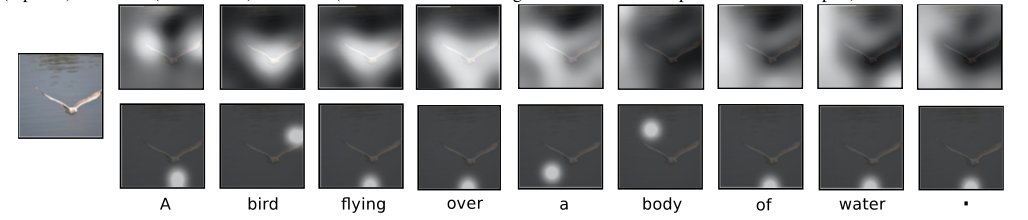
\includegraphics[scale=0.4]{Imgs/show1.png}
\caption{نحوه عمل‌کرد الگوریتم در تغییر توجه بصری بصری و کلمه تولید شده در هر نقطه. \cite{xu2015show}}
\label{fig:show1}
\end{figure}  
  
  در تمام تصاویر، محدوده‌های روشن‌تر، محدوده‌هایی هستند که در آن‌ها ضریب میانگین‌گیری بیشتر بوده و توجه بیشتری در محاسبات روی آن‌ها متمرکز شده است. شکل \ref{fig:show2} چند نمونه از تصاویر را نمایش می‌دهد که در آن‌ها توجه بصری روی یک جسم منجر به تولید کلمه دقیق متناظر آن جسم شده است. کلمه تولید شده در شرح نهایی تولید شده برای تصویر در زیر هر تصویر نمایش داده شده است.

\begin{figure}[h]
\centering
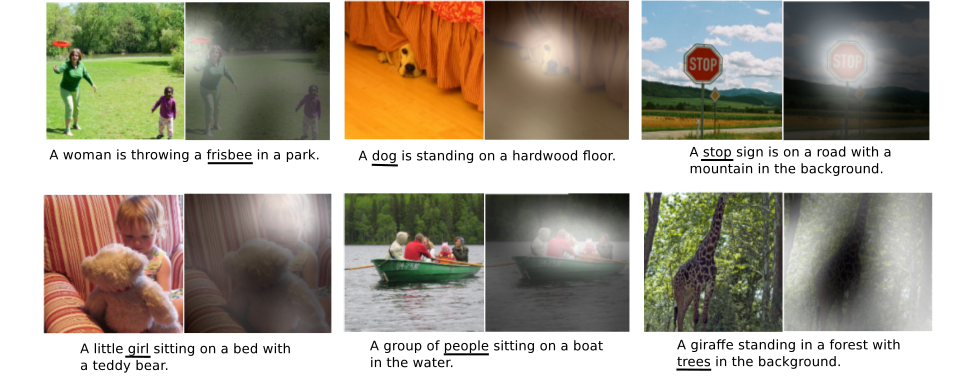
\includegraphics[scale=0.5]{Imgs/show2.png}
\caption{چند نمونه از تصاویر که در آن‌ها توجه بصری روی یک جسم منجر به تولید کلمه دقیق متناظر شده است\cite{xu2015show}. }
\label{fig:show2}
\end{figure}

  به علاوه، شکل \ref{fig:show3} نمایش‌دهنده شرایطی است که در آن کلمه تولید شده متناظر توجه بصری بصری نیست. با استفاده از بصری‌سازی محل توجه بصری و کلمه تولید شده در هر مرحله، می‌توان به راحتی مشاهده کرد که کلمه تولید شده متناظر کدام نقطه از تصویر،‌ نامناسب است.
  
  \begin{figure}[h]
  \centering
  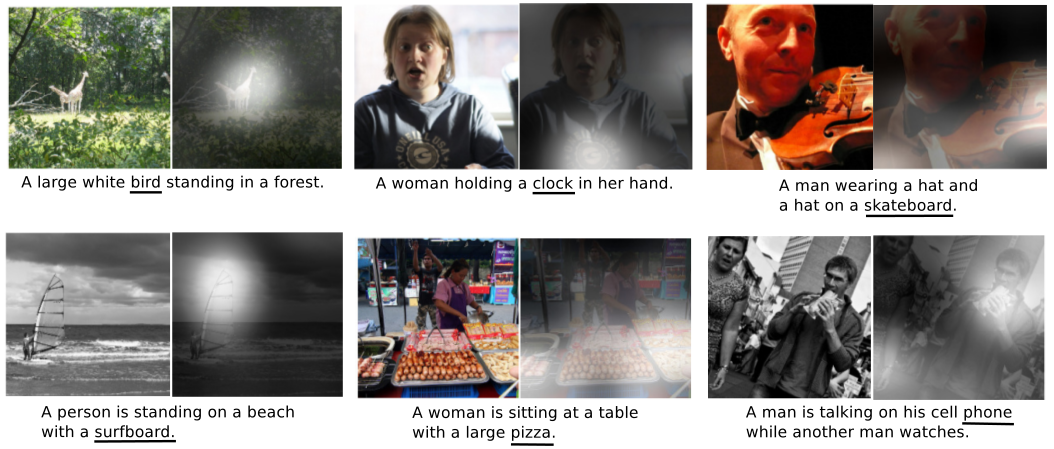
\includegraphics[scale=0.4]{Imgs/show3.png}
  \caption{نمونه‌هایی از تولید کلمات نامناسب مطابق با نقاط توجه استفاده شده در مدل‌\cite{xu2015show}}
  \label{fig:show3}
  \end{figure}
    
علاوه بر موارد فوق، نمونه‌ای از بررسی تمام مراحل تولید شرح متناظر صحنه برای یک تصویر را در حالت‌های استفاده از توجه بصری سخت در شکل \ref{fig:show4} و توجه بصری نرم در شکل \ref{fig:show5} قابل مشاهده است. هر کلمه تولید شده در هر مرحله در کنار میزان فعال‌سازی شبکه مربوط به آن کلمه نمایش داده شده است.

\begin{figure}[h]
\centering 
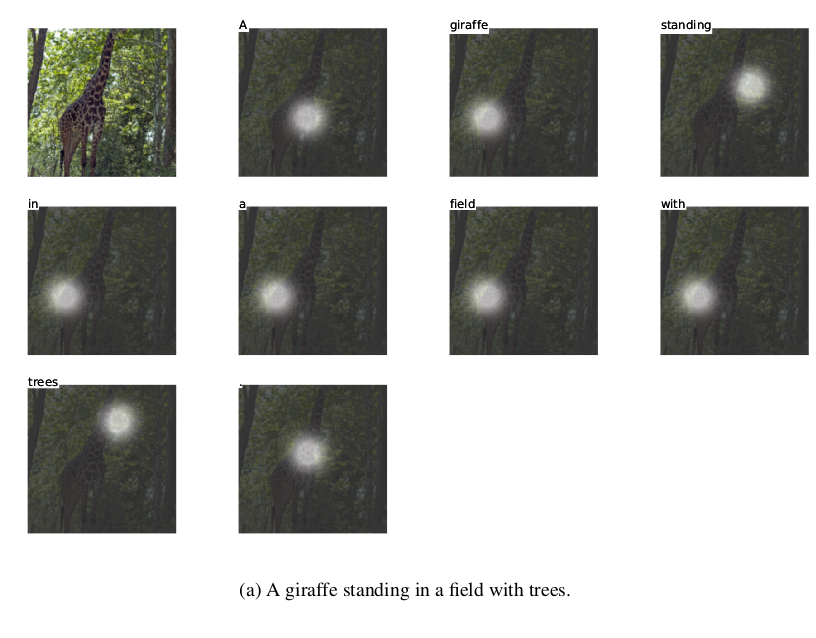
\includegraphics[scale=0.5]{Imgs/show4.png}
\caption{فرایند تولید شرح متناظر تصویر با استفاده از توجه بصری سخت \cite{xu2015show}}
\label{fig:show4}
\end{figure}


\begin{figure}[h]
\centering 
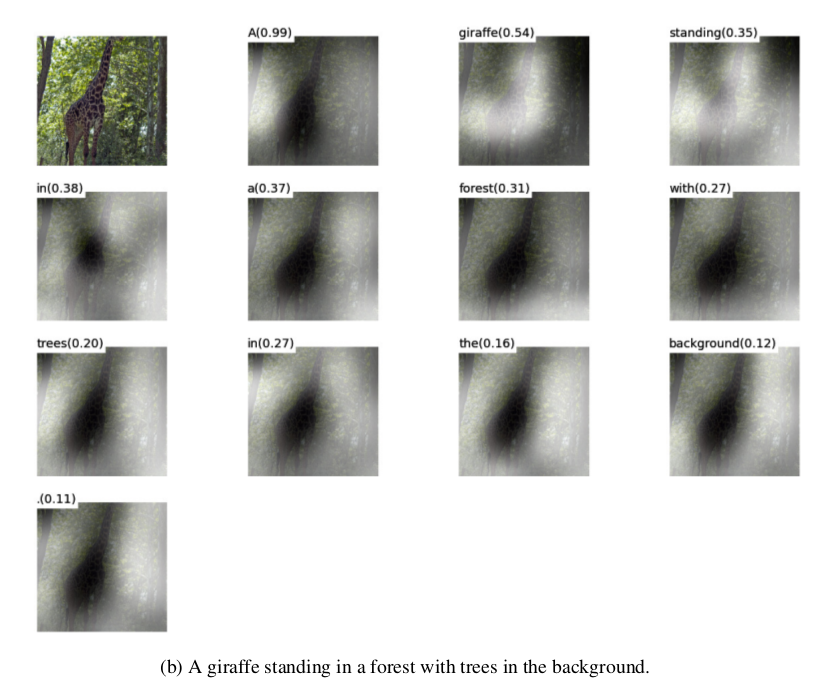
\includegraphics[scale=0.5]{Imgs/show5.png}
\caption{فرایند تولید شرح متناظر تصویر با استفاده از توجه بصری نرم \cite{xu2015show}}
\label{fig:show5}
\end{figure}


\subsection{فعالیت‌های مشابه دیگر}
استفاده از توجه بصری در حوزه تولید شرح متناظر تصویر، از سال 2015، توجه بسیاری از پژوهش‌گران را به خود جلب نموده است و پژوهش‌های زیادی با استفاده از این ایده سعی در تولید جمله برای تصاویر، ویدئو‌ها، صوت و انواع ورودی‌های مشابه نموده‌اند. همین‌طور در حوزه ترجمه ماشینی، نسخه‌های متفاوت و متنوعی از این ایده برای دست‌یابی به ترجمه‌های بهتر ارائه شده‌اند.
\\
یکی از پژوهش‌هایی که در این زمینه برای بهبود عمل‌کرد ترجمه ماشینی با استفاده از نقطه توجه ارائه شده است، پژوهشی است که آقای منینگ و همکارانش در سال 2015 ارائه دادند\cite{luong2015effective}.  در این پژوهش، که بر روی مجموعه‌داده \lr{WMT} که شامل جملات انگلیسی و معادل آلمانی آن‌ها است اجرا شده، از یک ساختار پشته‌ای مطابق شکل \ref{fig:5-abnmt} استفاده شده است. در این ساختار، برای آموزش، جمله انگلیسی و معادل آلمانی آن به یک‌دیگر الصاق شده و ساختار انکودر-دیکودری با هم آموزش می‌بینند. سپس با دریافت ورودی جمله انگلیسی یا آلمانی، معادل آن‌ها تولید می‌شود.



\begin{figure}[h]
\centering
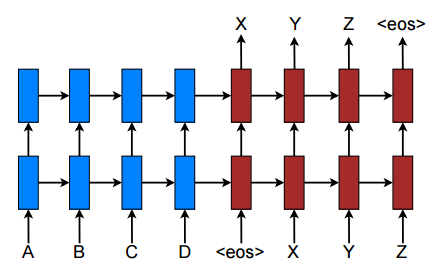
\includegraphics[scale=0.8]{Imgs/abnmt.png}
\caption{ساختار پشته‌ای ارائه شده در \cite{luong2015effective}}
\label{fig:5-abnmt}
\end{figure}

در پژوهش ارائه شده نیز مانند پژوهشی که آقای بنجیو در سال 2015 در حوزه ترجمه ماشینی انجام دادند، دو نوع توجه محاسبه و مورد آزمایش قرار گرفته است. توجه اول که معادل توجه نرم است، تحت عنوان توجه سراسری\enfootnote{Global Attention} و توجه دوم که معادل توجه سخت است، تحت عنوان توجه ناحیه‌ای\enfootnote{Local Attention} مطرح شده‌اند. در این آزمایش هم مشابه نتایج پژوهش \cite{xu2015show} توجه ناحیه‌ای، در بسیاری موارد عمل‌کرد بهتری نسبت به توجه سراسری از خود نشان داده‌است.
\\
پژوهش مشابهی در حوزه پرسش و پاسخ بصری توسط ایده مشابه پژوهش \cite{luong2015effective} در سال 2016 توسط آقای ینگ و همکارانش در \cite{yang2016stacked} ارائه شده است. در این پژوهش، بردار ویژگی تصویر به شرح متناظر آن که در مجموعه‌داده موجود است، الصاق شده و ساختار انکودر-دیکودری به شکل مشابهی آموزش می‌بیند. سپس با ورود یک تصویر جدید، بردار ویژگی آن به ساختار داده شده و جمله مرتبط با تصویر جدید توسط ساختار تولید می‌گردد.
\\
آقای بنجیو در پژوهش \cite{cho2015describing} در سال 2015، چارچوب کاری‌ای را مبتنی بر استفاده از نقطه توجه ارائه کردند که قابل استفاده در حوزه‌های ترجمه ماشینی، تولید شرح متناظر تصویر، توصیف ویدئو و گفتار است. در این پژوهش، علاوه بر ارائه یک روش برای محاسبه نقطه توجه بصری و استخراج بردار ویژگی با استفاده از بردارهای حاشیه‌نویسی، صحبت‌هایی در مورد امکان انتقال یادگیری در چارچوب ارائه شده انجام شده است. در این پژوهش در مورد هر یک از چهار حوزه‌ای که ذکر شد، صحبت شده و نحوه استفاده از چارچوب کاری در هر یک از این حوزه‌ها تبیین شده است. همین‌طور در این پژوهش اثبات شده است که استفاده از مکانیزم نقطه توجه، این امکان را به مدل می‌دهد که به طور بدون نظارت، رابطه هم‌ترازی بین بخش‌های ورودی و خروجی را یاد بگیرد تا بتوان از این ویژگی در انتقال یادگیری استفاده نمود. نتایج استفاده از این چارچوب کاری در حوزه‌های مختلف بهتر از روش‌های دیگر گزارش شده است. شکل \ref{fig:5-abedfw} ساختار چارچوب را در حوزه تولید شرح متناظر تصویر نمایش می‌دهد.

\begin{figure}[h]
\centering
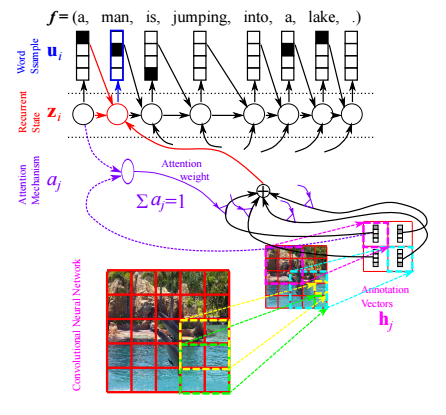
\includegraphics[scale=0.6]{Imgs/abedfw.png}
\caption{ساختار چارچوب کاری ارائه شده در \cite{cho2015describing} در حوزه تولید شرح متناظر تصویر}
\label{fig:5-abedfw}
\end{figure}



\subsection{جمع‌بندی}

چارچوب کاری انکودر-دیکودر یکی از اصلی‌ترین چارچوب‌های کاری در حوزه ترجمه ماشینی و پیرو آن تولید شرح متناظر تصویر به شمار می‌رود. انکودر در این چارچوب کاری وظیفه نگاشت ورودی به فضای معنا و دیکودر وظیفه نگاشت فضای معنا به فضای خروجی را بر عهده دارد. در حوزه ترجمه ماشینی معمولا از یک شبکه عصبی حافظه کوتاه‌مدت بلند به عنوان دیکودر استفاده می‌شود. این شبکه عصبی با دریافت کلمات جمله ورودی به ترتیب، بردار حالت مخفی خود را به‌روز‌رسانی می‌نماید. در نهایت می‌توان از این بردار به عنوان بردار حاصل نگاشت جمله ورودی به فضای معنا استفاده نمود.
\\
دیکودر در این چارچوب کاری با دریافت بردار ویژگی تولید شده توسط دیکودر، عمل تولید خروجی را برعهده خواهد داشت. در حوزه ترجمه ماشینی معمولا یک شبکه عصبی بازگشتی برای دیکودر می‌تواند مورد استفاده قرار بگیرد. به طور معمول، بردار ویژگی تولید شده توسط انکودر، به عنوان یک ورودی به دیکودر داده می‌شود و دیکودر در هر مرحله با تولید یک کلمه به عنوان خروجی، بردار حالت مخفی خود را به‌روزرسانی نموده و با استفاده از بردار حالت مخفی جدید، اقدام به تولید کلمه جدید می‌نماید.
\\
یکی از محدودیت‌های جدی فرایند مذکور این است که بردار ویژگی فقط یک بردار با طول ثابت است و اولا انکودر باید بتواند تمام اطلاعات قابل استخراج را تنها در این بردار جاسازی نماید و ثانیا دیکودر باید بتواند تمام اطلاعات مورد نیاز خود برای تولید کلمه و جمله را فقط از همین یک بردار استخراج نماید. این مشکل، پژوهش‌گران را بر آن داشت تا بردار ویژگی را از یک بردار با طول ثابت به یک دنباله بردار با طول ثابت و تعداد متغیر تغییر دهند. 
\\
به بردارهای ویژگی تولید شده در حالت جدید، حاشیه‌نویسی می‌گویند. این حاشیه‌نویسی‌ها باید دارای دو شرط زیر باشند:
\begin{enumerate}
\item دربرگیرنده تمام معنای ورودی باشند.
\item تمرکز بیشتری روی معنای یک بخش مشخص از ورودی داشته باشند.
\end{enumerate}
با در نظر گرفتن این ویژگی‌ها، دیکودر قادر خواهد بود تا هنگام تولید هر کلمه، روی معنای یک بخش از جمله تمرکز بیشتری داشته باشد و فقط از آن بخش برای تولید کلمه استفاده نماید. به این شکل، کلمات تولید شده شباهت بیشتری به ورودی خواهند داشت و ترجمه‌های بهتری حاصل خواهد شد. 
\\
در سال 2015، آقای بنجیو و همکارانش در پژوهش \cite{xu2015show} روشی ارائه دادند که در آن برای اولین بار از ایده استفاده از نقطه توجه در حوزه ترجمه ماشینی برای تولید شرح متناظر تصویر استفاده نمودند. در این پژوهش، از یک شبکه عصبی کانولوشنی به عنوان انکودر استفاده شده است. خروجی شبکه از لایه ماقبل آخر گرفته شده که منجر به ایجاد تعداد زیادی بردار ویژگی از تصویر می‌شود که هر کدام از این بردارهای ویژگی، از یک ناحیه از تصویر ایجاد شده‌اند و تمرکز بیشتری روی آن ناحیه داشته‌اند. 
\\
بدین ترتیب با استفاده از یک شبکه عصبی بازگشتی به عنوان دیکودر و استفاده از بردارهای حاشیه‌نویسی ایجاد شده توسط انکودر می‌توان به راحتی عملیات تولید شرح متناظر تصویر را انجام داد. تنها نکته‌ای که باید مشخص شود، چگونگی استفاده از بردارهای حاشیه‌نویسی است. در این پژوهش دو روش مختلف برای استفاده از بردارهای حاشیه‌نویسی مطرح شده است.
\\
روش اول موسوم به روش توجه سخت، روشی است که در آن فقط یک بردار حاشیه‌نویسی انتخاب شده و از آن برای تولید جمله استفاده می‌شود. در این روش به هر یک از بردارهای حاشیه‌نویسی توسط یک مدل که قبلا آموزش دیده است، یک وزن اختصاص می‌دهیم و سپس با توجه به وزن‌های تخصیص داده شده به هر بردار حاشیه‌نویسی، یکی از آن‌ها را به عنوان بردار ویژگی تصویر انتخاب کرده و از آن در مراحل بعدی استفاده می‌کنیم.
\\
روش دوم موسوم به روش توجه نرم، روشی است که در آن یک بردار ویژگی کلی از روی بردارهای حاشیه‌نویسی تولید شده و از آن بردار در مراحل بعدی استفاده می‌شود. برای تولید این بردار نیز مانند روش توجه سخت، ابتدا توسط یک مدل که از پیش‌آموزش دیده است، به هر یک از بردارهای حاشیه‌نویسی یک وزن اختصاص می‌دهیم. سپس می‌توان با محاسبه امید ریاضی بردارهای حاشیه‌نویسی با توجه به وزن هر یک از آن‌ها بردار ویژگی نهایی را برای تصویر تولید و از آن برای تولید جمله استفاده کرد.
\\
آزمایشات انجام شده روی این مدل نشان می‌دهد، معیار \lr{BlEU-1} حاصل از این روش با استفاده از توجه سخت معمولا از مدل توجه نرم بیش‌تر بوده است. مطابق با نتایج گزارش شده در این پژوهش، میزان امتیاز \lr{BLEU-1} حاصل توسط توجه سخت روی مجموعه‌داده‌های \lr{MS COCO}، \lr{Flickr30k}  و \lr{Flickr8k} به ترتیب برابر با 71.8، 66.9 و 67.0 است. این در حالیست که امتیاز حاصل توسط توجه نرم روی همین مجموعه‌های داده، به ترتیب برابر با 70.8، 66.7 و 67.0 و امتیاز کسب شده توسط مدل \lr{Log Bilinear} در بهترین حالت، به ترتیب برابر با 70.8، 60.0 و 65.6 بوده است. 
\\
مطابق با آزمایشات انجام‌شده، استفاده از توجه نرم، معیار \lr{METEOR} را نسبت به استفاده از توجه سخت افزایش می‌دهد. طبق نتایج گزارش‌شده در پژوهش، امتیاز \lr{METEOR} حاصل از توجه نرم به ترتیب روی مجموعه‌داده‌های \lr{Flickr8k}، \lr{Flickr30k} و \lr{MS COCO} برابر با 18.93، 18.49 و 23.90 بوده است. این در حالیست که امتیاز کسب‌شده توسط توجه سخت به ترتیب برابر با 20.30، 18.46 و 23.04 و امتیاز کسب‌شده توسط روش \lr{Log Bilinear} در بهترین حالت به ترتیب برابر است با 17.31، 16.88 و 20.03. این موضوع نشان می‌دهد با وجود این‌که جملات تولید شده توسط روش توجه سخت با در نظر گرفتن جملات موجود در مجموعه‌داده از امتیاز بالاتری نسبت به جملات تولید شده توسط توجه نرم برخوردارند؛ استفاده از توجه نرم، منجر به تولید جملات قابل قبول‌تری توسط انسان می‌شود.
\\
پژوهش‌های مختلفی از این ایده در حوزه‌های مختلف استفاده نموده‌اند که گزارش مختصری از تعدادی از این پژوهش‌ها ارائه شده است.

